\documentclass{assignment}
\ProjectInfos{光电子技术}{PHYS6651P}{2021-2022学年第一学期}{第八章作业}{}{陈稼霖}[https://github.com/Chen-Jialin]{SA21038052}

\begin{document}
\begin{prob}
    图示一种相位型光纤温度传感器原理图,从两光纤末端输出的两光波在空间叠加形成明暗相间的杨氏条纹. 当信号臂的温度发生变化时,输出两端光波的相位差发生改变($\Delta\varphi$)表示,于是屏上条纹发生移动,观测条纹移动数便可求得温度的变化量,并有公式如下:$\varphi/(\Delta T\cdot L)=2\pi/\lambda(\Delta n/\Delta T+n\Delta L/(L\Delta T))$. 如果光源 $\lambda=6328$ \AA,光纤的折射率 $n=1.456$,$\mathrm{d}n/\mathrm{d}T=10\times 10^{-6}/^{\circ}$C,$\alpha=\Delta L/(L\cdot\Delta T)=5\times 10^{-7}/^{\circ}$C,光纤长度 $L=1$ 米,求对应一个条纹间隔变化时的温度的变化.
\end{prob}
\begin{sol}
    
\end{sol}

\begin{prob}
    全光纤马赫-泽德(M-Z)滤波器通常是由两个 $3$ dB 耦合器连接而成,如下图所示,定向耦合器的传输矩阵为 $\begin{bmatrix}
        \sqrt{1-C}&-j\sqrt{C}\\
        -j\sqrt{C}&\sqrt{1-C}
    \end{bmatrix}$,光纤段的传输矩阵为 $\begin{bmatrix}
        \exp(-jk_0nl_1)&0\\
        0&\exp(-jk_0nl_2)
    \end{bmatrix}$,其中 $C$ 为耦合效率($3$ dB 相当于 $C=0.5$),$I_1$ 和 $I_2$ 为中间光纤臂长,设光场从 1 端输入,求从 3、4 端出射的光场振幅透射系数 $T_{13}$ 和 $T_{14}$ 及相邻透射峰之间的波长差.
    \begin{figure}[h]
        \centering
        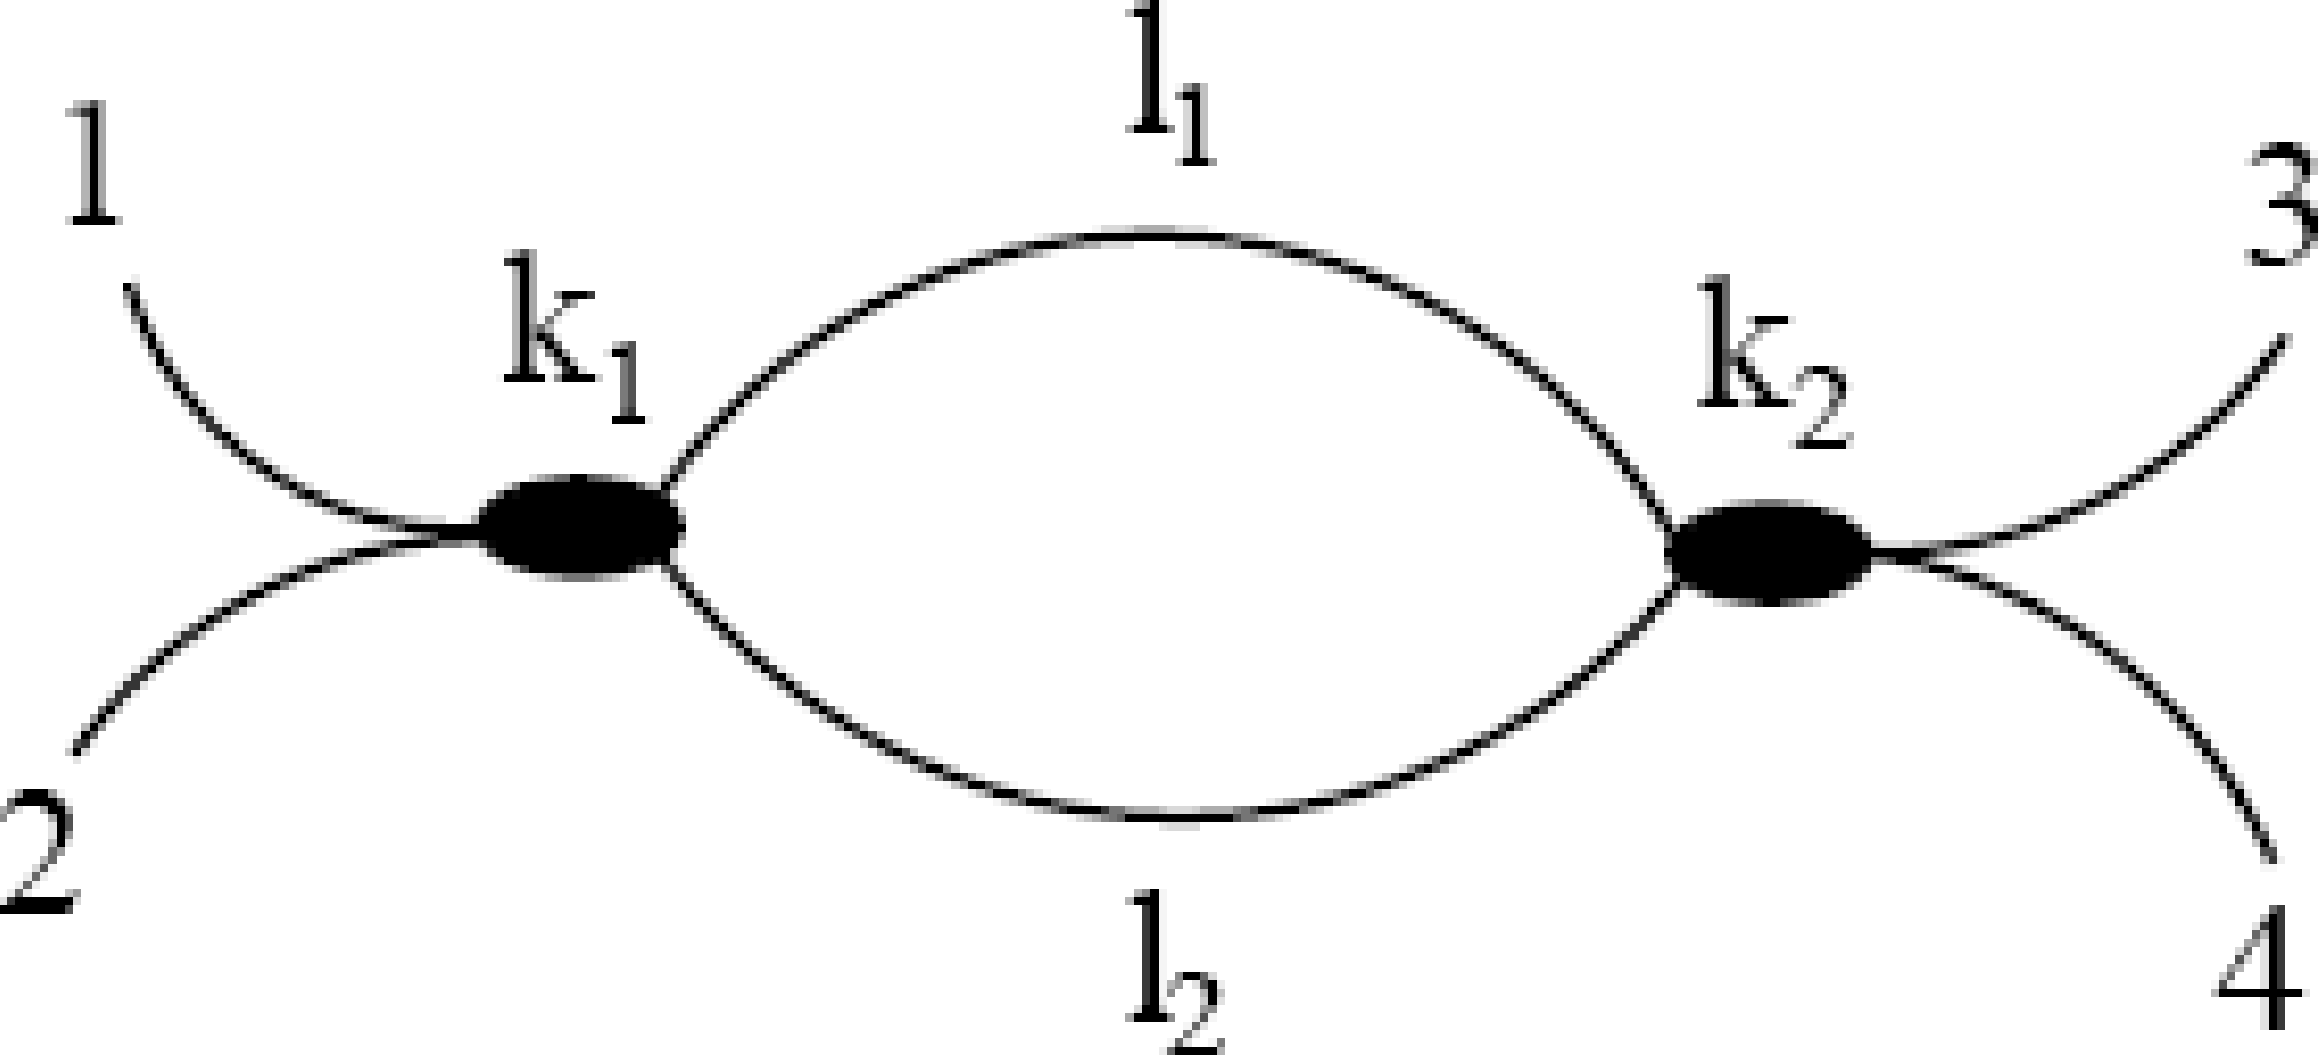
\includegraphics[width=.5\columnwidth]{4-3.png}
    \end{figure}
\end{prob}
\begin{sol}
    
\end{sol}
\end{document}